\documentclass[12pt]{article}

%%%%%%%%%%%%%%%%%%%%%%%%%%%%%%%%%%%%%%%%%%%%%%%%%%%%%%%%%%%%%%%%%%%%%%%%%%%%%%%%
%                           Package preset for homework
%%%%%%%%%%%%%%%%%%%%%%%%%%%%%%%%%%%%%%%%%%%%%%%%%%%%%%%%%%%%%%%%%%%%%%%%%%%%%%%%
% Miscellaneous
\usepackage[margin=1in]{geometry}
\usepackage[utf8]{inputenc}
\usepackage{indentfirst}
\usepackage{blindtext}
\usepackage{graphicx}
\usepackage{xr-hyper}
\usepackage{hyperref}
\usepackage{enumitem}
\usepackage{color}
\usepackage{float}
% Math
\usepackage{latexsym}
\usepackage{amsfonts}
\usepackage{amssymb}
\usepackage{amsmath}
\usepackage{commath}
\usepackage{amsthm}
\usepackage{bbold}
\usepackage{bm}
% Physics
\usepackage{physics}
\usepackage{siunitx}
% Code typesetting
\usepackage{listings}
% Citation
\usepackage[authoryear]{natbib}
\usepackage{appendix}
\usepackage[capitalize]{cleveref}
% Title & name
\title{Homework}
\author{Tien Vo}
\date{\today}


%%%%%%%%%%%%%%%%%%%%%%%%%%%%%%%%%%%%%%%%%%%%%%%%%%%%%%%%%%%%%%%%%%%%%%%%%%%%%%%%
%                   User-defined commands and environments
%%%%%%%%%%%%%%%%%%%%%%%%%%%%%%%%%%%%%%%%%%%%%%%%%%%%%%%%%%%%%%%%%%%%%%%%%%%%%%%%
%%% Misc
\sisetup{load-configurations=abbreviations}
\newcommand{\due}[1]{\date{Due: #1}}
\newcommand{\hint}{\textit{Hint}}
\let\oldt\t
\renewcommand{\t}[1]{\text{#1}}

%%% Bold sets & abbrv
\newcommand{\N}{\mathbb{N}}
\newcommand{\Z}{\mathbb{Z}}
\newcommand{\R}{\mathbb{R}}
\newcommand{\Q}{\mathbb{Q}}
\let\oldP\P
\renewcommand{\P}{\mathbb{P}}
\newcommand{\LL}{\mathcal{L}}
\newcommand{\FF}{\mathcal{F}}
\newcommand{\HH}{\mathcal{H}}
\newcommand{\NN}{\mathcal{N}}
\newcommand{\ZZ}{\mathcal{Z}}
\newcommand{\RN}[1]{\textup{\uppercase\expandafter{\romannumeral#1}}}
\newcommand{\ua}{\uparrow}
\newcommand{\da}{\downarrow}

%%% Unit vectors
\newcommand{\xhat}{\vb{\hat{x}}}
\newcommand{\yhat}{\vb{\hat{y}}}
\newcommand{\zhat}{\vb{\hat{z}}}
\newcommand{\nhat}{\vb{\hat{n}}}
\newcommand{\rhat}{\vb{\hat{r}}}
\newcommand{\phihat}{\bm{\hat{\phi}}}
\newcommand{\thetahat}{\bm{\hat{\theta}}}

%%% Other math stuff
\providecommand{\units}[1]{\,\ensuremath{\mathrm{#1}}\xspace}
% Set new style for problem
\newtheoremstyle{problemstyle}  % <name>
        {10pt}                   % <space above>
        {10pt}                   % <space below>
        {\normalfont}           % <body font>
        {}                      % <indent amount}
        {\bfseries\itshape}     % <theorem head font>
        {\normalfont\bfseries:} % <punctuation after theorem head>
        {.5em}                  % <space after theorem head>
        {}                      % <theorem head spec (can be left empty, 
                                % meaning `normal')>

% Set problem environment
\theoremstyle{problemstyle}
\newtheorem{problemenv}{Problem}[section]
\newenvironment{problem}[1]{%
  \renewcommand\theproblemenv{#1}%
  \problemenv
}{\endproblemenv}
% Set lemma environment
\newenvironment{lemma}[2][Lemma]{\begin{trivlist}
\item[\hskip \labelsep {\bfseries #1}\hskip \labelsep {\bfseries #2.}]}{\end{trivlist}}
% Set solution environment
\newenvironment{solution}{
    \begin{proof}[Solution]$ $\par\nobreak\ignorespaces
}{\end{proof}}
\numberwithin{equation}{problemenv}

%%% Page format
\setlength{\parindent}{0.5cm}
\setlength{\oddsidemargin}{0in}
\setlength{\textwidth}{6.5in}
\setlength{\textheight}{8.8in}
\setlength{\topmargin}{0in}
\setlength{\headheight}{18pt}

%%% Code environments
\definecolor{dkgreen}{rgb}{0,0.6,0}
\definecolor{gray}{rgb}{0.5,0.5,0.5}
\definecolor{mauve}{rgb}{0.58,0,0.82}
\lstset{frame=tb,
  language=Python,
  aboveskip=3mm,
  belowskip=3mm,
  showstringspaces=false,
  columns=flexible,
  basicstyle={\small\ttfamily},
  numbers=none,
  numberstyle=\tiny\color{gray},
  keywordstyle=\color{blue},
  commentstyle=\color{dkgreen},
  stringstyle=\color{mauve},
  breaklines=true,
  breakatwhitespace=true,
  tabsize=4
}
\lstset{
  language=Mathematica,
  numbers=left,
  numberstyle=\tiny\color{gray},
  numbersep=5pt,
  breaklines=true,
  captionpos={t},
  frame={lines},
  rulecolor=\color{black},
  framerule=0.5pt,
  columns=flexible,
  tabsize=2
}


\title{Homework 2: Phys 7320 (Spring 2022)}
\due{January 26, 2022}

\begin{document}
\maketitle
%%%%%%%%%%%%%%%%%%%%%%%%%%%%%%%%%%%%%%%%%%%%%%%%%%%%%%%%%%%%%%%%%%%%%%%%%%%%%%%
\begin{problem}{2.1}[A four-charge quadrupole]
A radiating quadrupole consists of a square of side $a$ with charge $\pm q$ at
alternate corners. The square rotates with angular velocity $\omega$ about an
axis normal to the plane of the square and through its center. Calculate the
quadrupole moments, the radiation fields, the angular distribution of radiation,
and the total radiated power, all in the long-wavelength approximation. What is
the frequency of radiation?
\begin{solution}
First, the monopole moment is just the total charge, which we know by the set up
that $Q=0$. Second, the four charge is in configuration such that they form two
dipoles, each with $p=qa$ but with opposite signs. So the total dipole moment is
also zero. Now, we calculate the quadrupole tensor
\begin{equation}
    Q_{ij}=\int(3x_ix_j-r^2\delta_{ij})\rho(\vb{x})d^3x 
\end{equation}
The trajectories of the charges as they rotate in the $(xy)$-plane around the
origin is
\begin{subequations}
    \begin{align}
        x_{1,n}&=r\cos\qty[\omega t+(n-1)\frac\pi2]\\
        x_{2,n}&=r\sin\qty[\omega t+(n-1)\frac\pi2]\\
        x_{3,n}&=0
    \end{align} 
\end{subequations}
for $n\in\qty{1,2,3,4}$ and $r=a/\sqrt2$ so that they make a square of
sidelength $a$. Thus,
\begin{align}
    \rho(\vb{x})&=q\qty[\delta(\vb{x}-\vb{x}_1)
    -\delta(\vb{x}-\vb{x}_2)
    +\delta(\vb{x}-\vb{x}_3)
    -\delta(\vb{x}-\vb{x}_4)
    ]\notag\\
            &=q\sum_{n=1}^4(-1)^{n-1}\delta(x_1-x_{1,n})
\delta(x_2-x_{2,n})\delta(x_3-x_{3,n})
\end{align}
Then the tensor elements can be written as
\begin{equation}\label{p1:Q}
    Q_{ij}=q\sum_{n=1}^4\qty(-1)^{n-1}\int (3x_ix_j-r^2\delta_{ij})
    \delta(x_1-x_{1,n})\delta(x_2-x_{2,n})\delta(x_3)dx_1dx_2dx_3
\end{equation}
First, because the quadrupole lies entirely in the $(xy)$-plane, $Q_{i3}=0$ for
all $i$. Plugging \eqref{p1:Q} into Mathematica, we can find the non-trivial
elements and write
\begin{equation}
    Q_{ij}=6qr^2\mqty(
    \cos2\omega t & \sin2\omega t & 0\\
    \sin2\omega t & -\cos2\omega t & 0\\
    0 & 0 & 0)=3qa^2\mqty(1&i&0\\i&-1&0\\0&0&0)e^{-2i\omega t}
\end{equation}
By definition (9.43, Jackson), the vector
\begin{align}
    \vb{Q}(\vb{n})
    &= Q_{ij}n_j\notag\\
    &=\frac{3qa^2}{r}e^{-2i\omega t}\qty[(x+iy)\xhat+(ix-y)\yhat]\notag\\
    &=\frac{3qa^2}{r}e^{-2i\omega t}(x+iy)(\xhat+i\yhat)\notag\\
    &=3qa^2e^{2i(\phi-\omega
    t)}\sin\theta\qty(\sin\theta\rhat+\cos\theta\thetahat+i\phihat)
\end{align}
and we can then calculate from (9.44, Jackson)
\begin{align}\label{p1:H}
    \vb{H}
    &=-\frac{ick^3}{24\pi}\frac{e^{ikr}}{r}\vb{n}\times\vb{Q}(\vb{n})\notag\\
    &=-\frac{ick^3qa^2}{8\pi}\frac{e^{i(kr-2\omega t-2\phi)}}{r}
    \sin\theta\qty(\cos\theta\phihat-i\thetahat)
\end{align}
and
\begin{equation}\label{p1:E}
    \vb{E}=Z_0\vb{H}\times\vb{n}
    =-\frac{iZ_0ck^3qa^2}{8\pi}\frac{e^{i(kr-2\omega t-2\phi)}}{r}
    \sin\theta\qty(\cos\theta\thetahat+i\phihat)
\end{equation}
From (9.45, Jackson), the antenna pattern is then
\begin{equation}
    \frac{dP}{d\Omega}
    =\frac{Z_0c^2k^6}{1152\pi^2}\abs{\qty[\vb{n}\times\vb{Q}(\vb{n})\times\vb{n}]}^2
    =\frac{Z_0c^2k^6q^2a^4}{128\pi^2}\qty(1-\cos^4\theta)
\end{equation}
and the total radiated power is
\begin{equation}
    P=\int\frac{dP}{d\Omega}d\Omega
    =\frac{Z_0c^2k^6q^2a^4}{64\pi}\int_0^\pi d\theta\sin\theta(1-\cos^4\theta)
    =\frac{Z_0c^2k^6q^2a^4}{40\pi}
\end{equation}
From the oscillatory term in \eqref{p1:H} and \eqref{p1:H}, the frequency of 
radiation is $2\omega$.

\end{solution}
\end{problem}
\newpage
%%%%%%%%%%%%%%%%%%%%%%%%%%%%%%%%%%%%%%%%%%%%%%%%%%%%%%%%%%%%%%%%%%%%%%%%%%%%%%%    
%%%%%%%%%%%%%%%%%%%%%%%%%%%%%%%%%%%%%%%%%%%%%%%%%%%%%%%%%%%%%%%%%%%%%%%%%%%%%%%
\begin{problem}{2.2}[An antenna: exact]
A thin linear antenna of length $d$ is excited in such a way that the sinusoidal
current makes a full wavelength of oscillation.

(a) Calculate exactly the power radiated per unit solid angle and plot the
angular distribution of radiation.

(b) Determine the total power radiated and find a numerical value for the
radiation resistance.
\begin{solution}
(a) Given the current $I=I_0\sin\qty(2\pi z/d) e^{-i\omega t}$ where $2\pi
/d=2\pi/\lambda=k$, we can write the current density in the antenna as
\begin{equation}\label{p2:J}
    \vb{J}=I_0\sin\qty(kz)e^{-i\omega t}\delta(x)\delta(y)\zhat
\end{equation}
Then from (9.8, Jackson), the vector potential is
\begin{align}
    \vb{A}
    &=\zhat\frac{\mu_0I_0}{4\pi}\frac{e^{i(kr-\omega t)}}{r}
        \int d^3x'\sin(kz')\delta(x')\delta(z')e^{-ik\vb{n}\vdot\vb{x}'}
        \notag\\
    &=\zhat\frac{\mu_0I_0}{4\pi}\frac{e^{i(kr-\omega t)}}{r}
    \int_{-\pi/k}^{\pi/k}dz'\sin(kz')e^{-ikz'\cos\theta}\notag\\
    &=-i\zhat\frac{\mu_0I_0}{2\pi}\frac{e^{i(kr-\omega t)}}{kr}\frac{\sin(\pi
    u)}{1-u^2}
\end{align}
where $u=\cos\theta$. Then the magnetic field is
\begin{align}
    \vb{H}
    =\frac{ik}{\mu_0}\vb{n}\times\vb{A}
    =\frac{I_0}{2\pi}\frac{e^{i(kr-\omega t)}}{r}\frac{\sin\pi
    u}{1-u^2}\vb{n}\times\zhat
    =\frac{I_0}{2\pi}\frac{e^{i(kr-\omega t)}}{r^2}\frac{\sin\qty(\pi
    u)}{1-u^2}\qty(y\xhat-x\yhat)
\end{align}
Now, we write $\vb{H}=H\vb{w}$ where $\vb{w}=(y\xhat-x\yhat)$. By definition, 
the antenna pattern is
\begin{align}
    \frac{dP}{d\Omega}
    &=\frac12\Re\qty[r^2\vb{n}\vdot\qty(\vb{E}\times\vb{H}^\ast)]\notag\\
    &=\frac{Z_0}{2}\Re\qty{
    \vb{x}\vdot\qty[\qty(\vb{H}\times\vb{x})\times\vb{H}^\ast]}\notag\\
    &=\frac{Z_0}{2}\abs{H}^2\qty{\vb{x}\vdot\qty[(\vb{w}\times\vb{x})\times\vb{x}]}\notag\\
    &=\frac{Z_0}{2}\abs{H}^2\qty(x^2+y^2)r^2\notag\\
    &=\frac{Z_0}{2}\abs{H}^2r^4(1-u^2)\notag\\
    &=\frac{Z_0I_0^2}{8\pi^2}\frac{\sin^2(\pi u)}{1-u^2}
\end{align}
where we have solved the term in the curly bracket with Mathematica.
Fig~\ref{fig:p2} shows a plot of $dP/d\Omega$.
\begin{figure}[H]
    \centering
    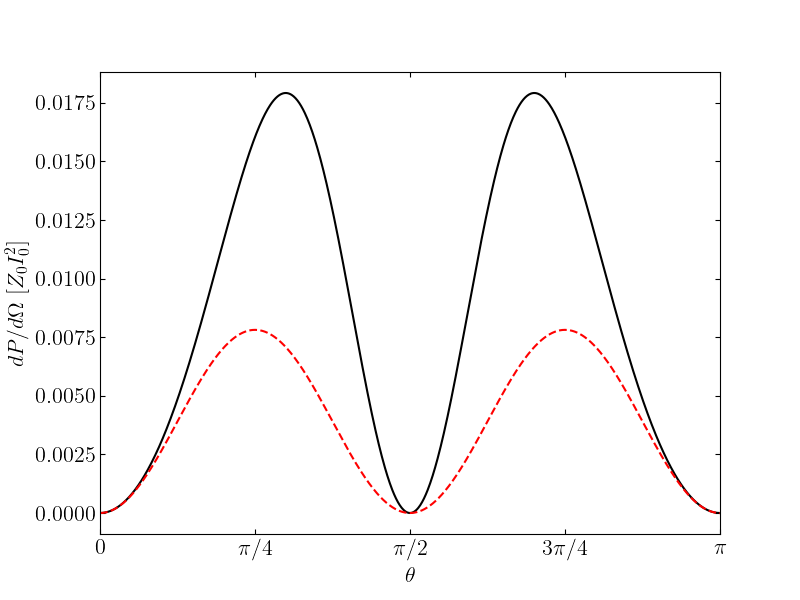
\includegraphics[width=0.8\textwidth]{p2.png}
    \caption{Angular distribution of the radiation pattern using exact
    derivation (solid black) and multipole expansion (dashed red).}
    \label{fig:p2}
\end{figure}

(b) From the previous results, the total power is
\begin{equation}
    P=\frac{Z_0I_0^2}{4\pi}\int_0^1du\frac{\sin^2(\pi u)}{1-u^2} 
    \approx \frac{0.779}{4\pi}Z_0I_0^2
    \approx 0.062 Z_0I_0^2
\end{equation}
The radiation resistance is
\begin{equation}
    R_\text{rad}=\frac{2P}{I_0^2}
    =\frac{0.779}{2\pi}Z_0\approx46.7\,\unit{\Omega}
\end{equation}
\end{solution}
\end{problem}
\newpage
%%%%%%%%%%%%%%%%%%%%%%%%%%%%%%%%%%%%%%%%%%%%%%%%%%%%%%%%%%%%%%%%%%%%%%%%%%%%%%%
%%%%%%%%%%%%%%%%%%%%%%%%%%%%%%%%%%%%%%%%%%%%%%%%%%%%%%%%%%%%%%%%%%%%%%%%%%%%%%%
\begin{problem}{2.3}[An antenna: multipole approximation]
Treat the linear antenna of Problem 9.16 by the multipole expansion method.

(a) Calculate the multipole moments (electric dipole, magnetic dipole, and
electric quadrupole) in the long wave-length approximation.

(b) Compare the shape of the angular distribution of radiated power for the
lowest nonvanishing multipole with the exact distribution of Problem 9.16.

(c) Determine the total power radiated for the lowest multipole and the
corresponding radiation resistance using both multipole moments from part (a).
Compare with Problem 9.16b. Is there a paradox here?
\begin{solution}
(a) From continuity equation, we can calculate the charge density using
\eqref{p2:J}
\begin{equation}
    \rho=\frac1{i\omega}\frac{\partial J_z}{\partial z}
    =\frac{k}{i\omega}I_0\cos(kz)e^{-i\omega t}\delta(x)\delta(y)
\end{equation}
Then the electric dipole moment is
\begin{equation}
    \vb{p}=\int d^3x'\vb{x}'\rho(\vb{x}')
    =\frac{k}{i\omega}I_0e^{-i\omega t}\zhat\int_{-d/2}^{d/2}z'\cos(kz')dz'
    =\vb{0}
\end{equation}
The magnetic dipole moment is
\begin{equation}
    \vb{m}=\frac12\int d^3x'(\vb{x}'\times\vb{J}') 
    =\frac12 I_0e^{-i\omega t}\int
    d^3x'\sin(kz)\delta(x')\delta(y')(y'\xhat-x'\yhat)
    =\vb{0}
\end{equation}
Finally, we calculate the quadrupole tensor
\begin{equation}
    Q_{ij}=\frac{k}{i\omega}I_0e^{-i\omega t}\int(3x_ix_j-r^2\delta_{ij}) 
    \cos(kx_3)\delta(x_1)\delta(x_2)dx_1dx_2dx_3
\end{equation}
where we have switched to using $(x_1,x_2,x_3)$ instead of $(x,y,z)$ for
convenience. Note that by symmetry (the antenna lies on the $z$-axis), all the 
off-diagonal terms vanish. Then we get
\begin{equation}
    Q_{33}=\frac{k}{i\omega}I_0e^{-i\omega
    t}\int_{-d/2}^{d/2}2x_3^2\cos(kx_3)dx_3
    =i\frac{8\pi I_0}{\omega k^2}e^{-i\omega t}
\end{equation}
and $Q_{11}=Q_{22}=-(1/2)Q_{33}$ so that $Q_{ij}$ is traceless.

(b) From the previous results, the angular distribution is
\begin{equation}
    \frac{dP}{d\Omega}
    =\frac{Z_0c^2k^6}{512\pi^2}\abs{Q_{33}}^2\sin^2\theta\cos^2\theta
    =\frac{Z_0I_0^2}{32}\sin^2\theta\cos^2\theta
\end{equation}
For a plot of this, see Fig~\ref{fig:p2}. The angular distribution is still 
four-lobe, but the intensity is smaller and the locations of the maxima are 
shifted.

(c) Integrating the distribution from (b), we get
\begin{equation}
    P=\frac{\pi}{16}Z_0I_0^2\int_0^\pi\sin^3\theta\cos^2\theta d\theta
    =\frac{\pi}{60}Z_0I_0^2
    \approx0.052 Z_0I_0^2
\end{equation}
and the radiation resistance is
\begin{equation}
    R_\text{rad}=\frac{2P}{I_0^2}=\frac{\pi}{30}Z_0=39.45\,\unit{\Omega}
\end{equation}
These values are a bit lower than the results in Problem 2. But the total power
is not too far from the exact solution. The discrepancy is only $\sim16\%$. The
rest might be due to higher order terms.
\end{solution}
\end{problem}
%%%%%%%%%%%%%%%%%%%%%%%%%%%%%%%%%%%%%%%%%%%%%%%%%%%%%%%%%%%%%%%%%%%%%%%%%%%%%%%
\end{document}
